\documentclass[tikz,border=5pt]{standalone}
% v3: data-led scientific illustration grammar. No dashboard cards or banners.
\usepackage{fix-cm}
\usepackage{amsmath,amssymb,graphicx}
\usepackage{tikz}
\usetikzlibrary{positioning,calc,fit,backgrounds,patterns,decorations.pathreplacing}
\renewcommand{\familydefault}{\sfdefault}
\definecolor{Ink}{HTML}{203848}
\definecolor{Muted}{HTML}{657884}
\definecolor{Rule}{HTML}{D2DDE3}
\definecolor{Observed}{HTML}{4E7897}
\definecolor{Teal}{HTML}{318E83}
\definecolor{Orange}{HTML}{C98542}
\definecolor{PaleBlue}{HTML}{EAF1F6}
\definecolor{PaleTeal}{HTML}{E8F3F0}
\definecolor{PaleOrange}{HTML}{FBF1E7}
\definecolor{GrayFill}{HTML}{F1F4F6}
\newcommand{\figfont}{\sffamily\fontsize{9.5}{11.5}\selectfont}
\newcommand{\figsmall}{\sffamily\fontsize{9}{10.5}\selectfont}
\tikzset{
 every node/.style={font=\figfont,text=Ink,inner sep=2pt},
 label/.style={font=\figfont,align=center},
 small/.style={font=\figsmall,text=Muted,align=center},
 panelletter/.style={font=\sffamily\bfseries\fontsize{10}{12}\selectfont,anchor=west},
 operator/.style={draw=Rule,fill=white,line width=.65pt,minimum height=.55cm,align=center,inner sep=4pt},
 flow/.style={->,>=stealth,draw=Ink!85,line width=.75pt},
 weight/.style={->,>=stealth,draw=Muted,dashed,line width=.65pt},
 axis/.style={->,>=stealth,draw=Muted,line width=.5pt},
 hair/.style={draw=Rule,line width=.5pt},
 sum/.style={circle,draw=Ink,fill=white,line width=.65pt,minimum size=12pt,inner sep=0pt},
}
% Illustrative 4x5 target table, not learned weights or experimental measurements.
% State 0: missing white; 1: initializer gray; 2: missing values restored in teal.
% Coordinates span [0,1.55] x [0,1.24]. No Other column is implied in this glyph.
\newcommand{\DataGrid}[1]{%
 \foreach \r in {0,...,3}{\foreach \c in {0,...,4}{%
  \pgfmathtruncatemacro{\tone}{25+mod(\r*17+\c*23,55)}
  \pgfmathtruncatemacro{\miss}{(\r==0&&\c==3)||(\r==1&&\c==0)||(\r==2&&\c==2)}
  \ifnum\miss=1
   \ifnum#1=0 \fill[white] (\c*.31,\r*.31) rectangle ++(.31,.31);
   \else\ifnum#1=1 \fill[Muted!22] (\c*.31,\r*.31) rectangle ++(.31,.31);
   \else \fill[Teal!65] (\c*.31,\r*.31) rectangle ++(.31,.31);\fi\fi
  \else \fill[Observed!\tone] (\c*.31,\r*.31) rectangle ++(.31,.31);\fi
  \draw[white,line width=.7pt] (\c*.31,\r*.31) rectangle ++(.31,.31);
 }}
 \draw[draw=Rule,line width=.55pt] (0,0) rectangle (1.55,1.24);
}
% A C-channel token is shown as a compact stack of editable vector strips.
\newcommand{\ChannelStrip}[1]{%
 \foreach \j in {0,...,7}{\pgfmathtruncatemacro{\tone}{25+mod(\j*17,55)}
  \fill[#1!\tone] (\j*.12,0) rectangle ++(.10,.43);}
}
\newcommand{\MaskGrid}{%
 \foreach \r in {0,...,3}{\foreach \c in {0,...,4}{%
  \pgfmathtruncatemacro{\miss}{(\r==0&&\c==3)||(\r==1&&\c==0)||(\r==2&&\c==2)}
  \ifnum\miss=1 \fill[white] (\c*.31,\r*.31) rectangle ++(.31,.31);
  \else \fill[Observed!55] (\c*.31,\r*.31) rectangle ++(.31,.31);\fi
  \draw[white,line width=.7pt] (\c*.31,\r*.31) rectangle ++(.31,.31);}}
 \draw[draw=Rule,line width=.55pt] (0,0) rectangle (1.55,1.24);
}
% Four parts x three real visits plus one padded row. Arrows identify axes,
% not numerical/learned attention weights. Mode 0 temporal; mode 1 feature.
\newcommand{\AxisGrid}[1]{%
 \fill[PaleBlue] (0,0) rectangle (1.28,1.28);
 \ifnum#1=0 \fill[Observed!22] (.32,.32) rectangle (.64,1.28);
 \else \fill[Teal!23] (0,.64) rectangle (1.28,.96);\fi
 \fill[GrayFill] (0,0) rectangle (1.28,.32);
 \foreach \i in {0,...,4}{
  \draw[draw=white,line width=.75pt] (\i*.32,0) -- (\i*.32,1.28);
  \draw[draw=white,line width=.75pt] (0,\i*.32) -- (1.28,\i*.32);}
 \draw[draw=Rule,line width=.5pt] (0,0) rectangle (1.28,1.28);
 \ifnum#1=0
  \draw[<->,>=stealth,draw=Observed,line width=1pt] (.48,.44) -- (.48,1.16);
 \else
  \draw[<->,>=stealth,draw=Teal,line width=1pt] (.12,.80) -- (1.16,.80);\fi
}

% Exact installed CM size: avoid the shared 8.5 pt request substituting to 8 pt.
\renewcommand{\figsmall}{\sffamily\fontsize{9}{10.5}\selectfont}
\begin{document}
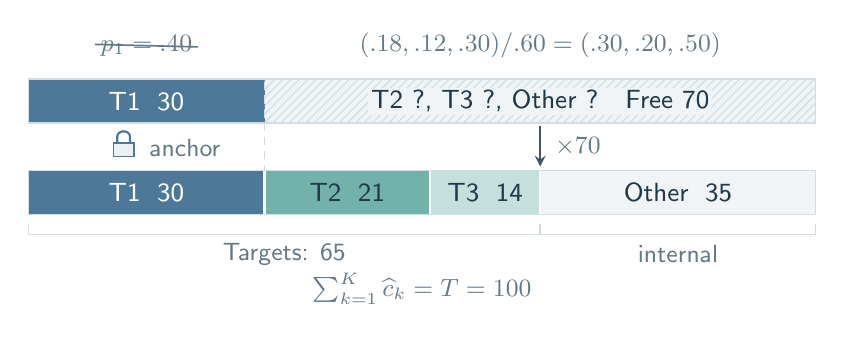
\begin{tikzpicture}[y=.8cm]
  % Original, exactly proportional illustration: 1 cm = 10 count units.
  % The anchor proposal is excluded; only the three free weights are normalized.
  \node[small] (excluded) at (1.5,3.88) {$p_1=.40$};
  \draw[draw=Muted,line width=.6pt]
    ($(excluded.west)+(0,.02)$) -- ($(excluded.east)+(0,-.02)$);
  \node[small] at (6.5,3.88)
    {$(.18,.12,.30)/.60=(.30,.20,.50)$};

  \fill[Observed] (0,2.65) rectangle (3,3.35);
  \path[fill=GrayFill] (3,2.65) rectangle (10,3.35);
  \path[pattern=north east lines,pattern color=Rule]
    (3,2.65) rectangle (10,3.35);
  \draw[hair] (0,2.65) rectangle (10,3.35);
  \node[label,text=white] at (1.5,3) {T1\; 30};
  \node[label,fill=GrayFill,inner sep=1pt] at (6.5,3.0)
    {T2 ?, T3 ?, Other ?\;\; Free 70};

  % Same anchor width and fill in both rows; the lock is an original vector glyph.
  \draw[hair,densely dashed] (3,1.2) -- (3,3.35);
  \path[draw=Observed,fill=PaleBlue,line width=.65pt]
    (1.08,2.12) rectangle (1.34,2.34);
  \draw[draw=Observed,line width=.8pt]
    (1.13,2.34) -- (1.13,2.44) arc (180:0:.08) -- (1.29,2.34);
  \node[small,anchor=west] at (1.46,2.25) {anchor};
  \draw[flow] (6.5,2.6) -- node[small,right=3pt] {$\times70$} (6.5,1.96);

  % Exact final partition: 30 + 21 + 14 + 35 = 100.
  \fill[Observed] (0,1.2) rectangle (3,1.9);
  \fill[Teal!68] (3,1.2) rectangle (5.1,1.9);
  \fill[Teal!28] (5.1,1.2) rectangle (6.5,1.9);
  \fill[GrayFill] (6.5,1.2) rectangle (10,1.9);
  \foreach \x in {3,5.1,6.5}
    \draw[white,line width=.9pt] (\x,1.2) -- (\x,1.9);
  \draw[hair] (0,1.2) rectangle (10,1.9);
  \node[label,text=white] at (1.5,1.55) {T1\; 30};
  \node[label] at (4.05,1.55) {T2\; 21};
  \node[label] at (5.8,1.55) {T3\; 14};
  \node[label] at (8.25,1.55) {Other\; 35};

  \draw[hair] (0,1.05) -- (0,.88) -- (6.5,.88) -- (6.5,1.05);
  \draw[hair] (6.5,1.05) -- (6.5,.88) -- (10,.88) -- (10,1.05);
  \node[small] at (3.25,.57) {Targets: 65};
  \node[small] at (8.25,.57) {internal};
  \node[small] at (5,.02) {$\sum_{k=1}^{K}\widehat c_k=T=100$};
\end{tikzpicture}
\end{document}
